\chapter{Практические задания}
\section{Задание}
\vspace{-0.7cm}
Используя хвостовую рекурсию, разработать эффективную программу,
(комментируя назначение аргументов), позволяющую:
\begin{enumerate}
	\item найти длину списка (по верхнему уровню);
	\item найти сумму элементов числового списка;
	\item найти сумму элементов числового списка, стоящих на нечетных позициях
	исходного списка (нумерация от 0);
\end{enumerate}
Убедиться в правильности результатов. Для одного из вариантов ВОПРОСА и одного из заданий составить таблицу,
отражающую конкретный порядок работы системы.

Код программы представлен на листинге \ref{lst:code}.
\newpage
\begin{lstlisting}[label=lst:code, basicstyle=\footnotesize, caption=Код программы]
domains
	list = integer*
predicates
	len_list(list, integer, integer).
	len_list(list, integer).
	
	sum_list(list, integer, integer).
	sum_list(list, integer).
	
	sum_odd_index_elems(list, integer, integer).
	sum_odd_index_elems(list, integer).
clauses
	len_list([_|Tail], Old_len, Len) :- 
						New_Len = Old_len + 1, !,
						len_list(Tail, New_len, Len).
	len_list([], Old_len, Old_len). 
	len_list(List, Len) :- len_list(List, 0, Len).
	
	sum_list([Head|Tail], Old_sum, Sum) :- 
						New_sum = Old_sum + Head, !,
						sum_list(Tail, New_sum, Sum).
	sum_list([], Old_sum, Old_sum).
	sum_list(List, Sum_elems) :- sum_list(List, 0, Sum_elems).
	
	sum_odd_index_elems([_, Head|Tail], Old_Sum, Sum) :- 
						New_sum = Old_sum + Head, !,
						sum_odd_index_elems(Tail, New_sum, Sum).
	sum_odd_index_elems([_], Old_sum, Old_sum) :- !.   							
	sum_odd_index_elems([], Old_sum, Old_sum).
	sum_odd_index_elems(List, Sum_elems) :- sum_odd_index_elems(List, 0, Sum_elems).
goal
	%найти длину списка (по верхнему уровню)
	%len_list([1, 2, 3], Len).
	
	%найти сумму элементов числового списка
	%sum_list([1, 2, 3], Sum_elems).
	
	%найти сумму элементов числового списка, стоящих на нечетных позициях
	%исходного списка (нумерация от 0)
	sum_odd_index_elems([1, 2, 3, 4, 5], Sum_elems).
\end{lstlisting}

Ниже на рисунках \ref{image:table_1} \ref{image:table_2} приведена таблица порядка поиска ответа для нахождения суммы элементов списка:
\begin{figure}[H]
	\centering{
		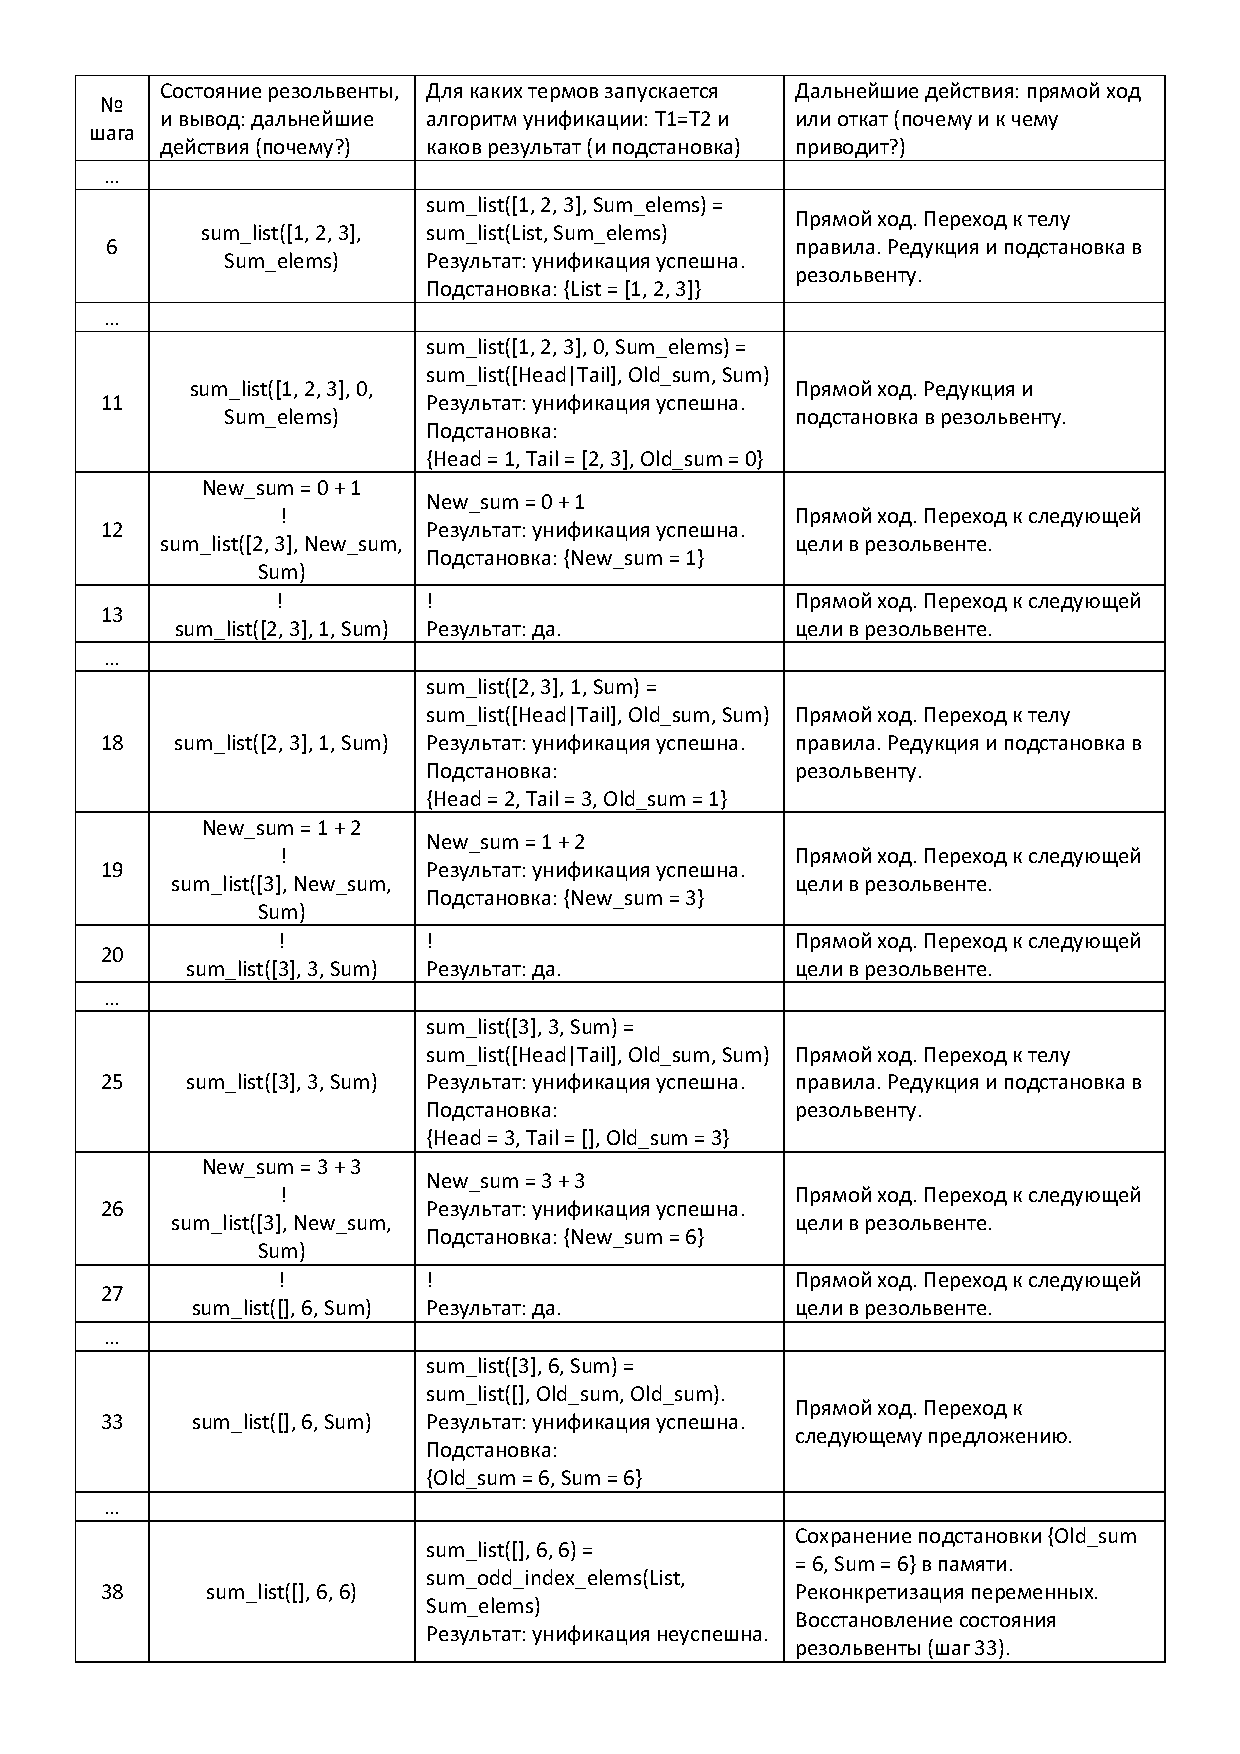
\includegraphics[scale=0.9]{images/table_7_1.pdf}
		\caption{Таблица порядка поиска ответов для нахождения суммы элементов списка.}
		\label{image:table_1}
	}
\end{figure}

\begin{figure}[H]
	\centering{
		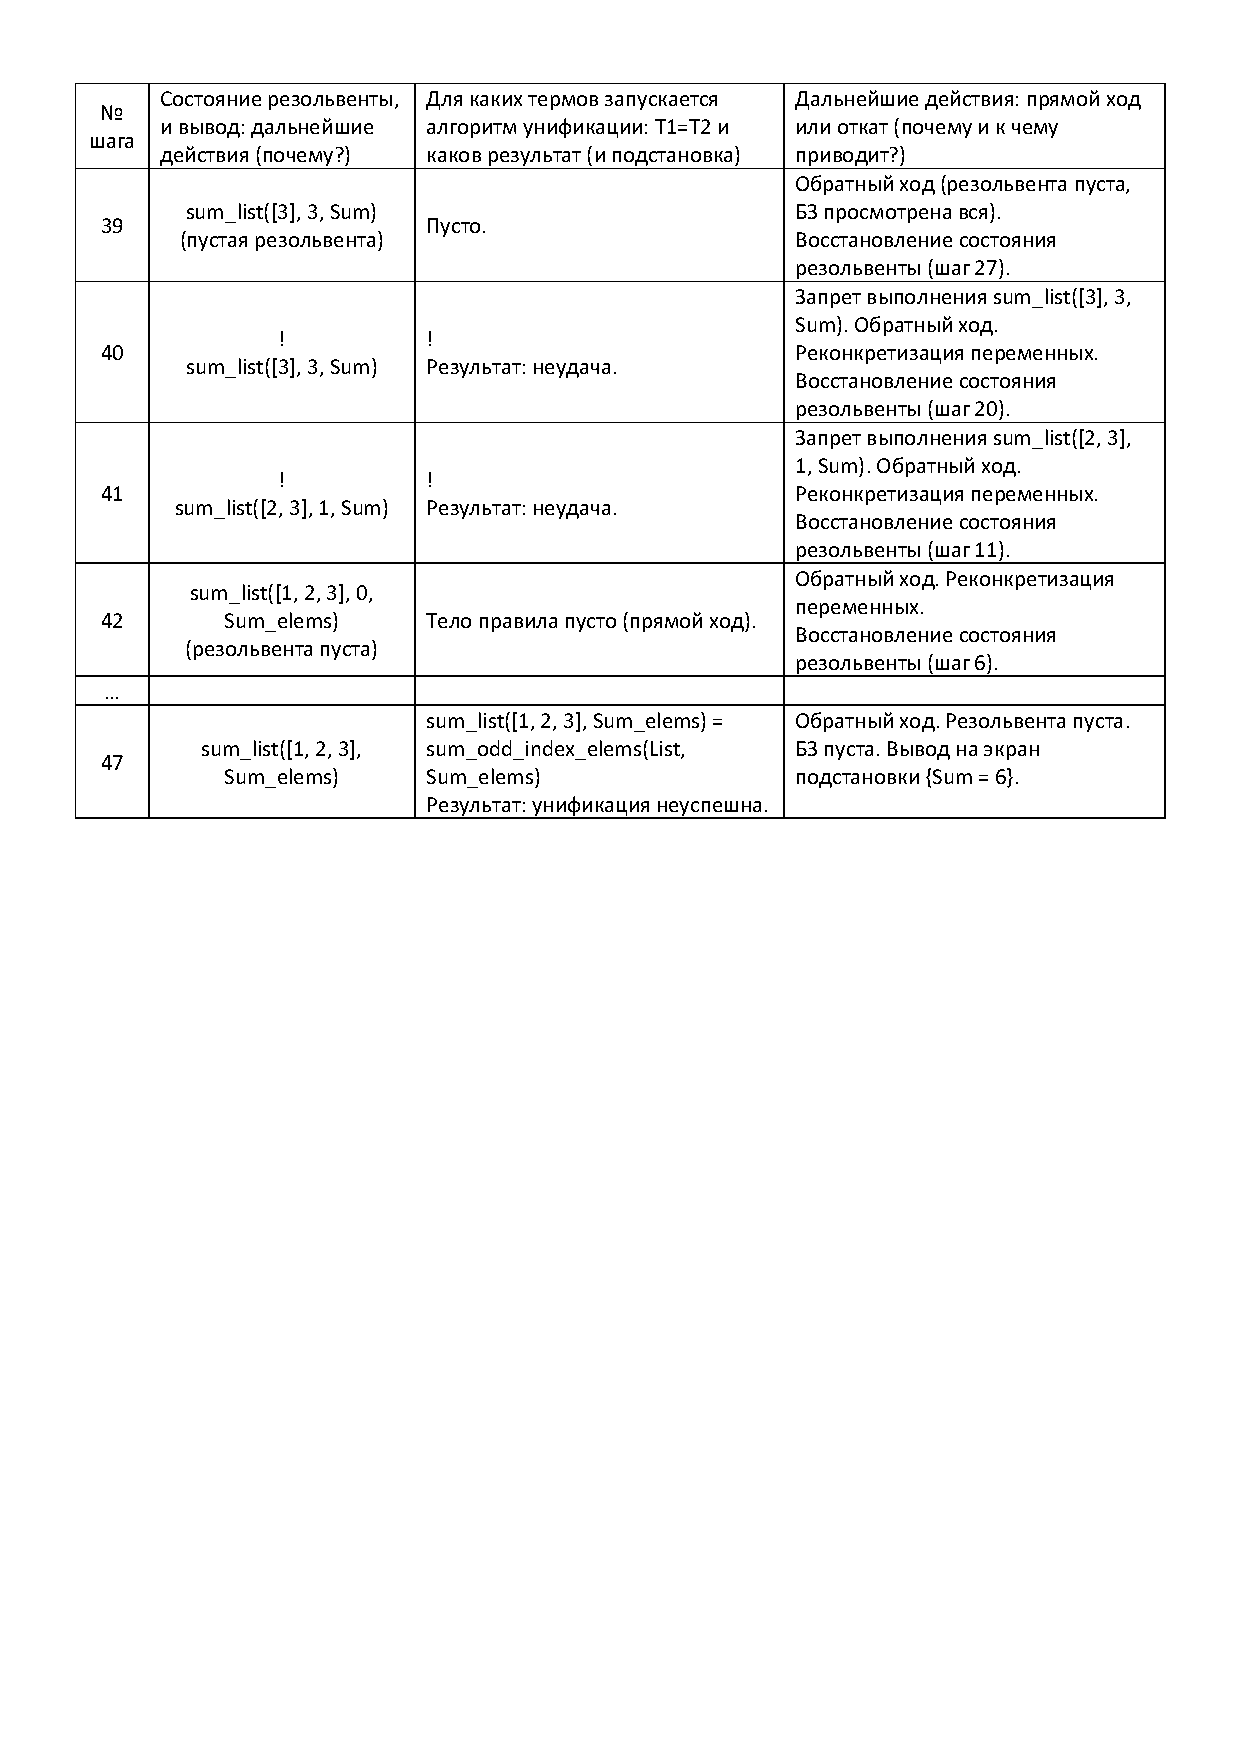
\includegraphics[scale=0.9]{images/table_7_2.pdf}
		\caption{Таблица порядка поиска ответов для нахождения суммы элементов списка (продолжение).}
		\label{image:table_2}
	}
\end{figure}